\chapter{Results}

From our measurements, the results varied a lot individually. Hence, grand average and further statistical analysis would not be well-applicable. In this section, individual results from selected participants are presented, including waveform morphology of the 14-channel measurements for both the HbO and HbR data. In addition, the regional analysis for the HbO data are also included in this section. Results from other measured participants are put in appendix.

First of all, our channels with the optode template are defined as shown in figure ~\ref{fig:ChannelDef}.

\begin{figure}[H]
  \centering
    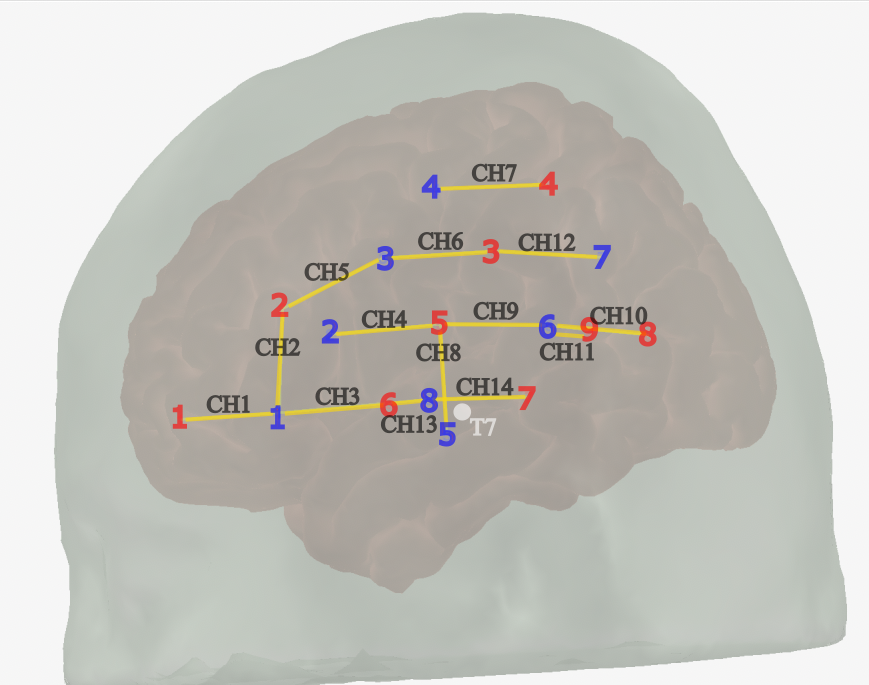
\includegraphics[scale=.45]{bilder/optode_ink.png}
  \caption{Channel Definition}
  \label{fig:ChannelDef}
\end{figure}


Our regions of interest (\acrshort{roi}) were defined as the following figure. The auditory cortex was in particular of our interest. Hence, channel 4, channel 8, and channel 9 together formed one region (ROI 2). The rest of the channels formed ROI 1. It was of our interest to compare how the response of the auditory cortex differ from the rest of the left brain hemisphere.


\vspace{1cm}
\begin{figure}[H]
  \centering
    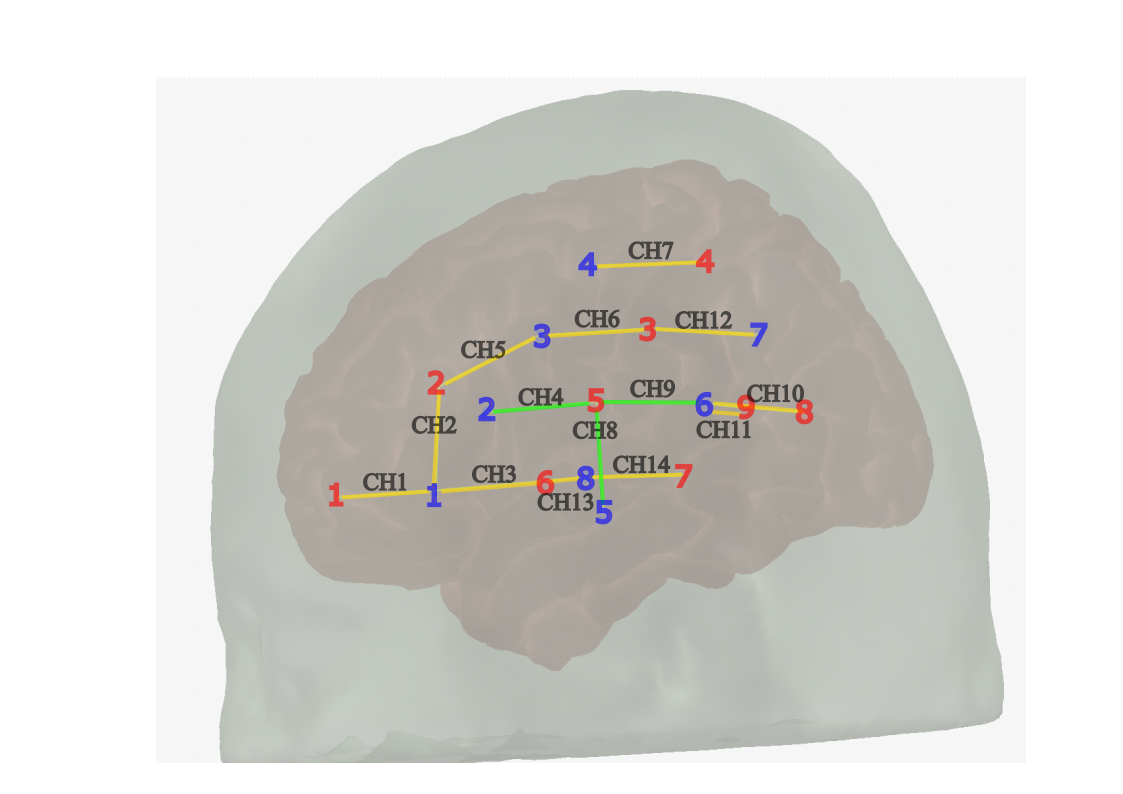
\includegraphics[scale=.45]{bilder/optode_roi_ink.png}
  \caption{ROI Definition}
\end{figure}


In the following plots, channels with invalid SCI are not taken into consideration, and hence are not be shown. Measurements in all channels are plotted in the same scale except for the two short channels, i.e. Channel 11 and 13, marked in thicker outlines. In all our measurements, the change in the dynamic hemoglobin response was significantly less in the short channels by more than a magnitude.
\newpage



\section {Participant 3}

\begin{figure}[H]
  \centering
    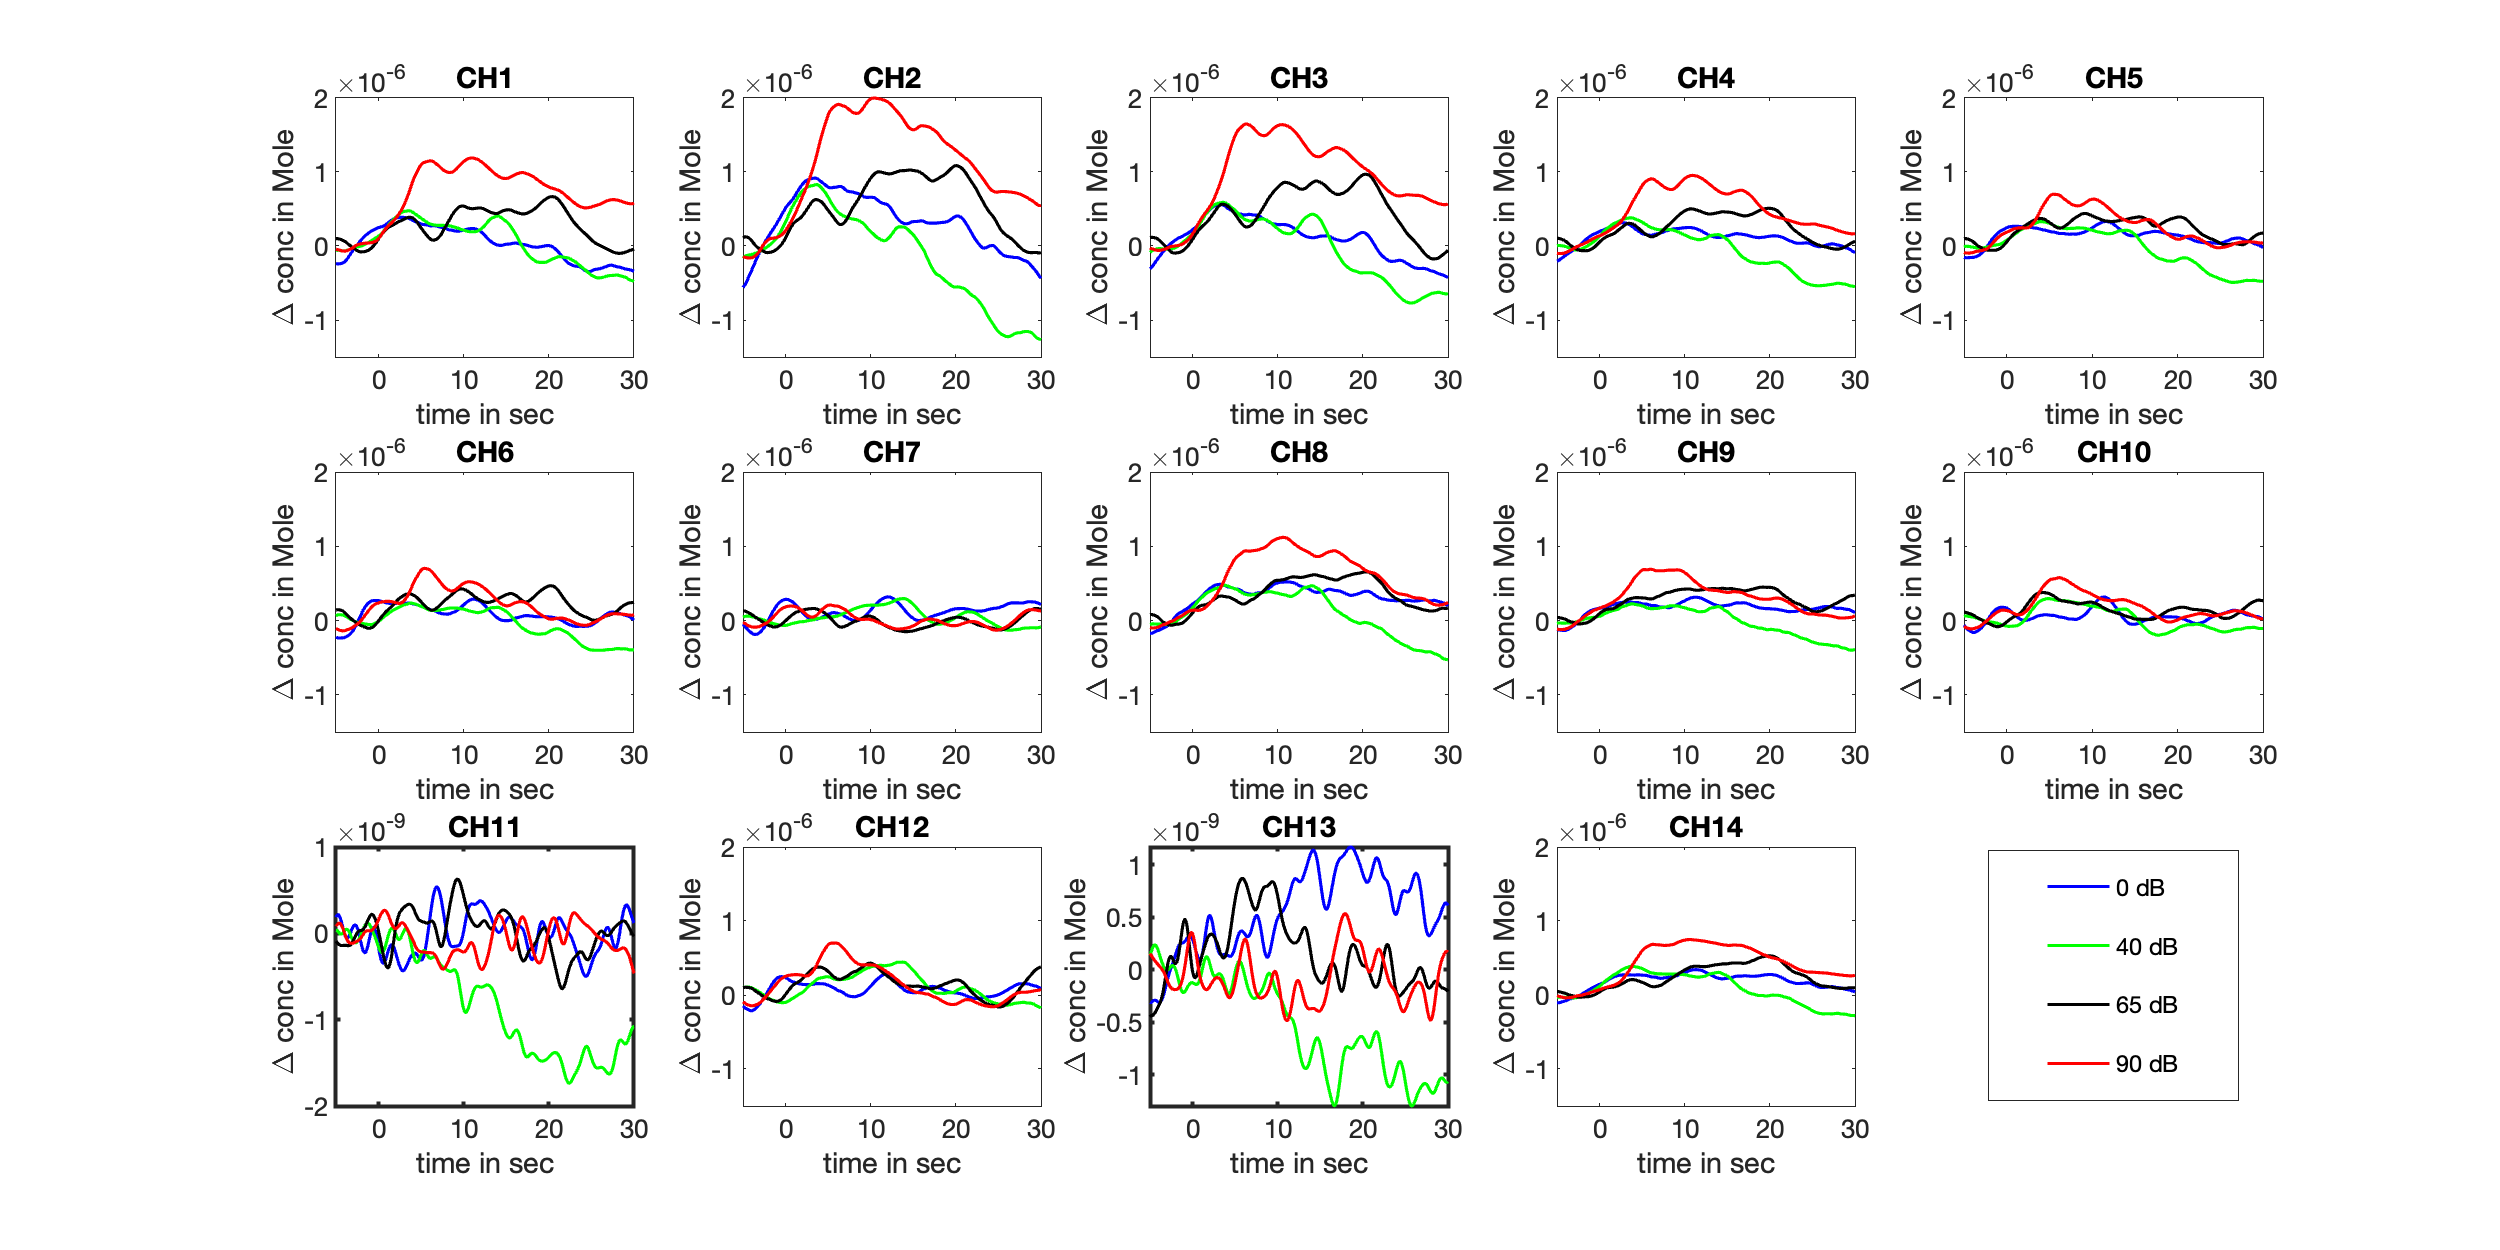
\includegraphics[scale=.4]{bilder/HbO_Mole/sub_jonas_s_HbO.png}
  \caption{HbO Measurement from participant 3.}
  \label{fig:somesignal}
  \medskip
  \footnotesize {Lines represent the block-averaged results over eight epochs. The averaged change of HbO concentration (in Mole) is plotted from 5 seconds before the start of the auditory stimuli to 30 seconds after the start of the stimuli. Four colours are used to differentiate the response from sound stimuli of different intensity levels.}
\end{figure}

For the HbO waveform morphology, tonic response could be observed in channel 1, 2, and 3, and phasic response could be observed in channel 10 and 12. \footnote {Tonic response refers to a sustained response, which activates during the course of the stimulus; while phasic response refers to a transient response with one or few action potentials at the onset of stimulus followed by accommodation. \citep {Wang2014IonicMU}} The sound stimuli of the greatest intensity resulted in the largest response in terms of magnitude in all the long channels. \\

The HbR measurement also showed separation from responses to stimuli of different SPLs. In most of the channel measurements, the loudest sound stimuli caused the most negative change of HbR concentration after 20 seconds from the start of sound stimuli. 

\newpage

\begin{figure}[H]
  \centering
    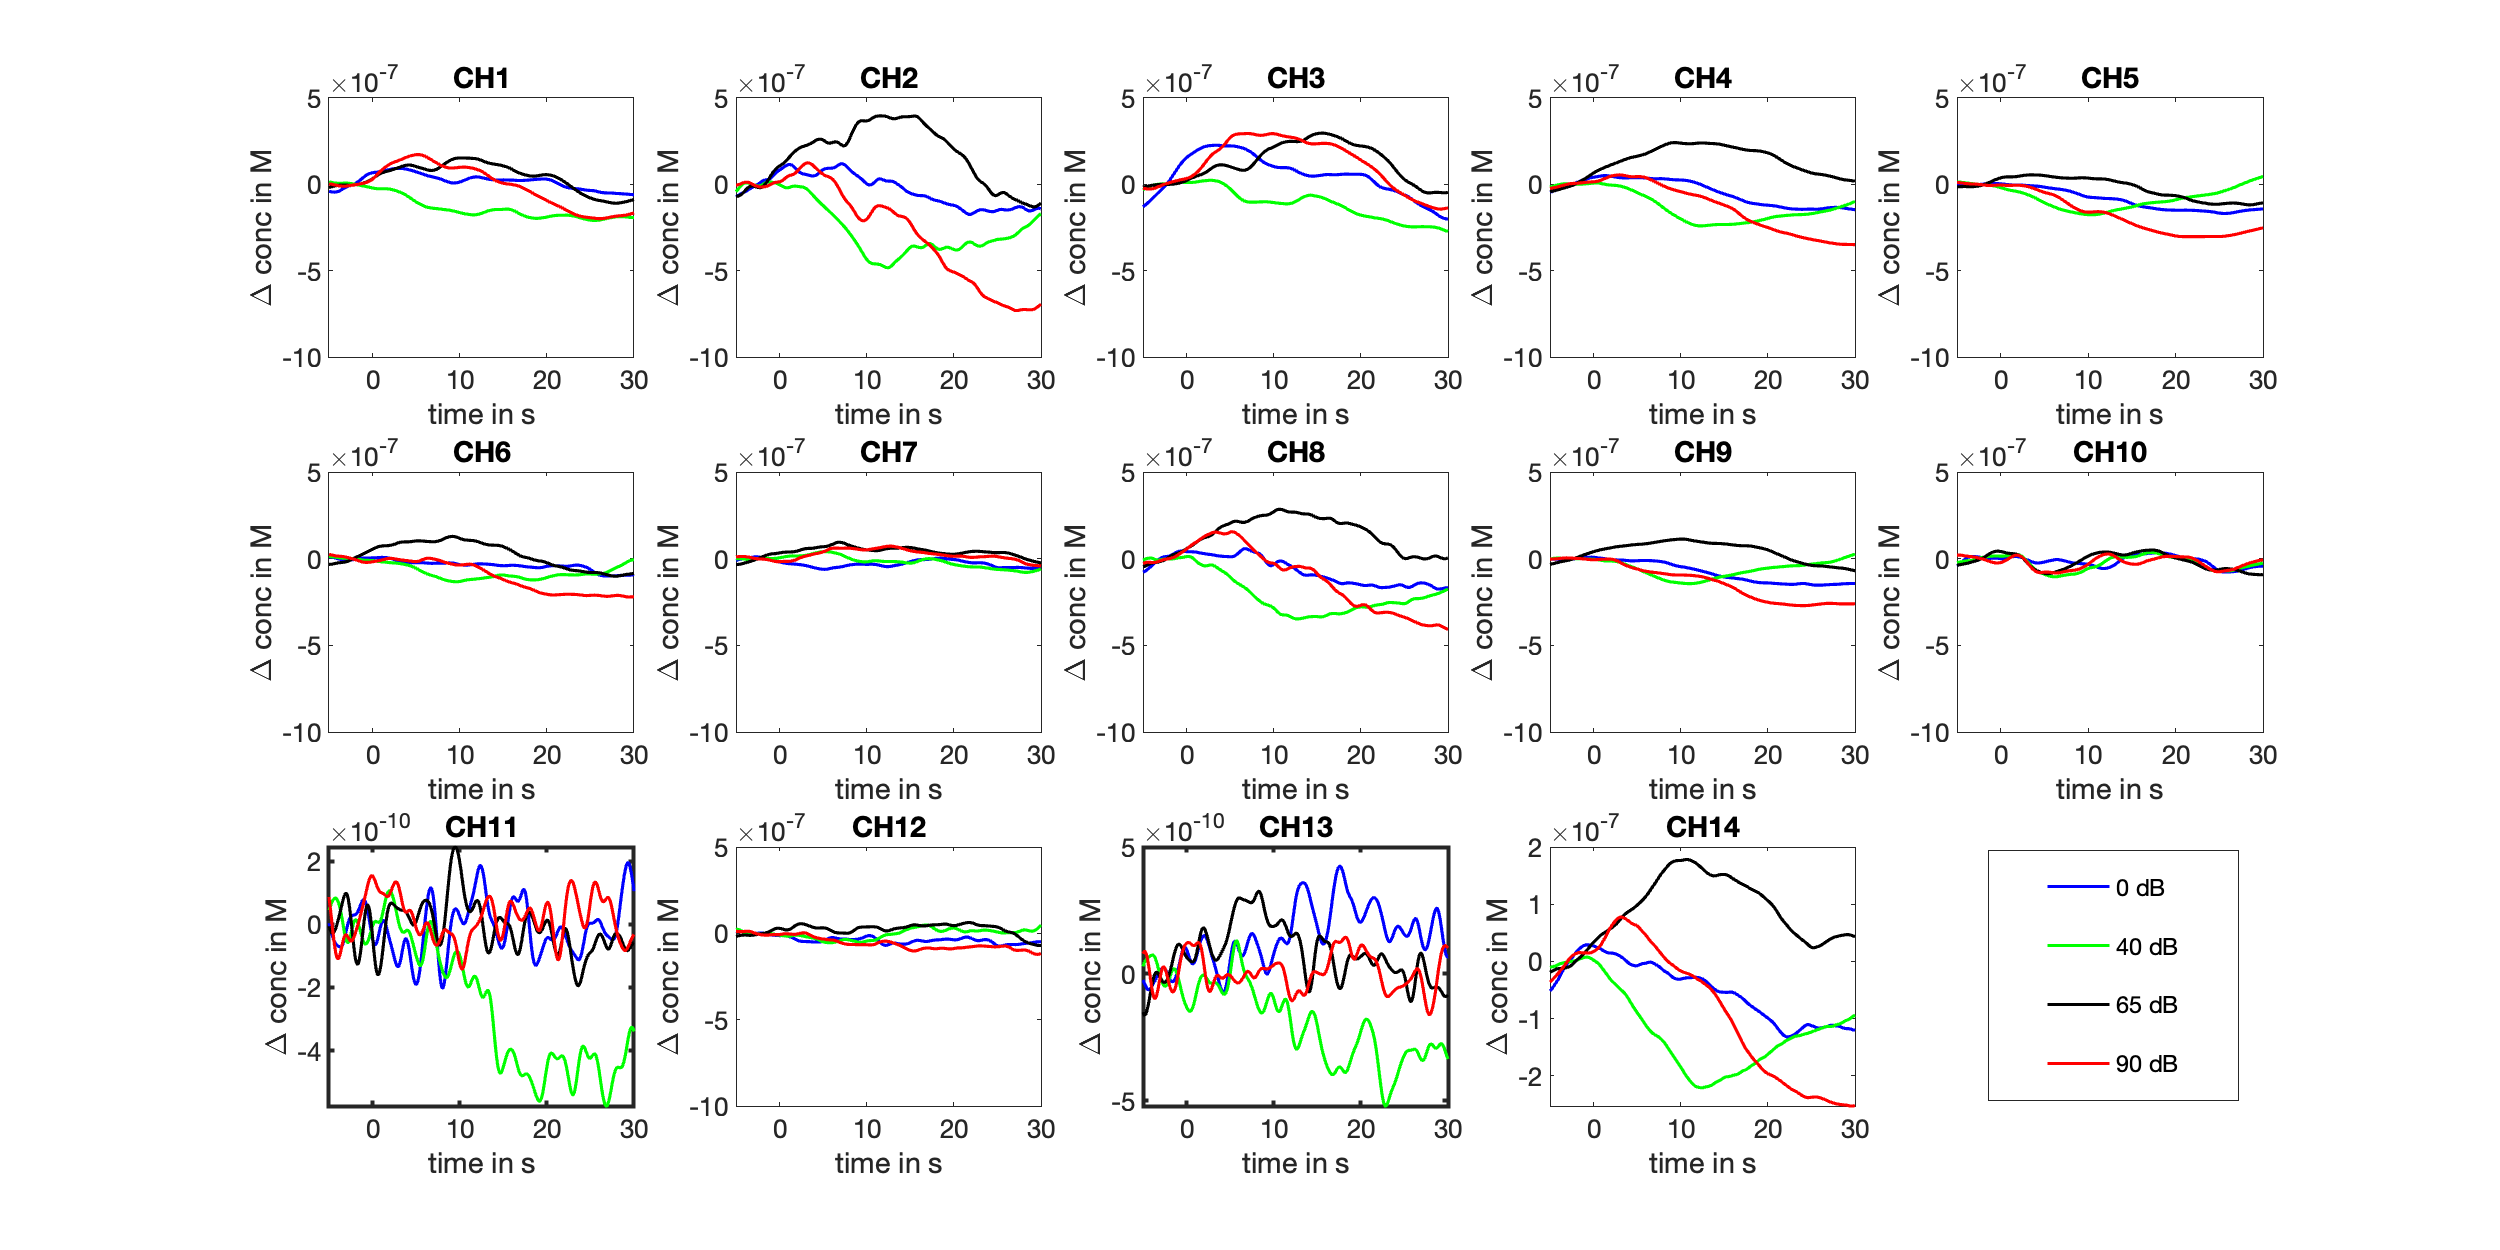
\includegraphics[scale=.4]{bilder/HbR_Mole/sub_jonas_s_HbR.png}
  \caption{HbR Measurement from participant 3.}
  \label{fig:somesignal}
  \medskip
  \footnotesize {Lines represent the block-averaged results over eight epochs. The averaged change of HbR concentration (in Mole) is plotted from 5 seconds before the start of the auditory stimuli to 30 seconds after the start of the stimuli. Four colours are used to differentiate the response from sound stimuli of different intensity levels.}
\end{figure}


\begin{figure}[H]
  \centering
    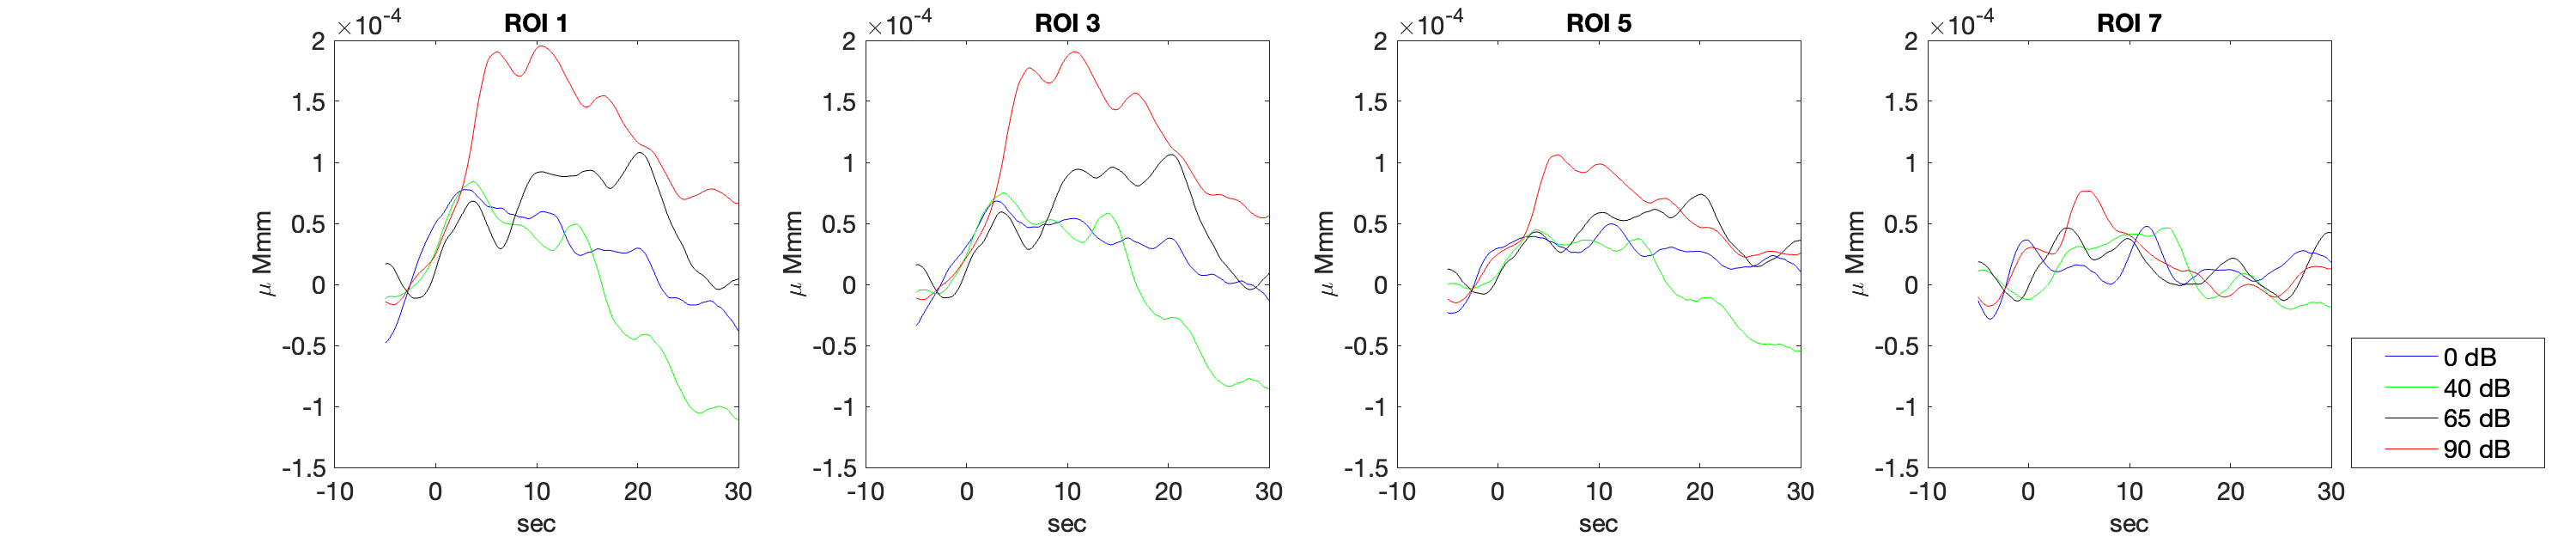
\includegraphics[scale=.3]{bilder/ROI/sub_jonas_s_HbO.png}
  \caption{ROI Measurement from participant  3.}
  \medskip
  \footnotesize {In every channel, the block-averaged HbO response over eight epochs was taken first before the mean HbO response in the whole region was calculated. The averaged change of HbO concentration (in Mole) for channels in the region is plotted from 5 seconds before the start of the auditory stimuli to 30 seconds after the start of the stimuli. Four colours are used to differentiate the response from sound stimuli of different intensity levels.}
\end{figure}

The results from this participant was the closest one to the results reported by Weder et al. 
\newpage


\section {Participant 4}
There were also some poor measurements even though the SCI is above the threshold 0.75. For example, in our case of participant 4, almost all channels showed barely any response except for channel 14, in which the measured data also appeared to be noisy. One potential reason was due to the thick dark hair of the participant that resulted in more light absorption, which affected the result greatly.

\begin{figure}[H]
  \centering
    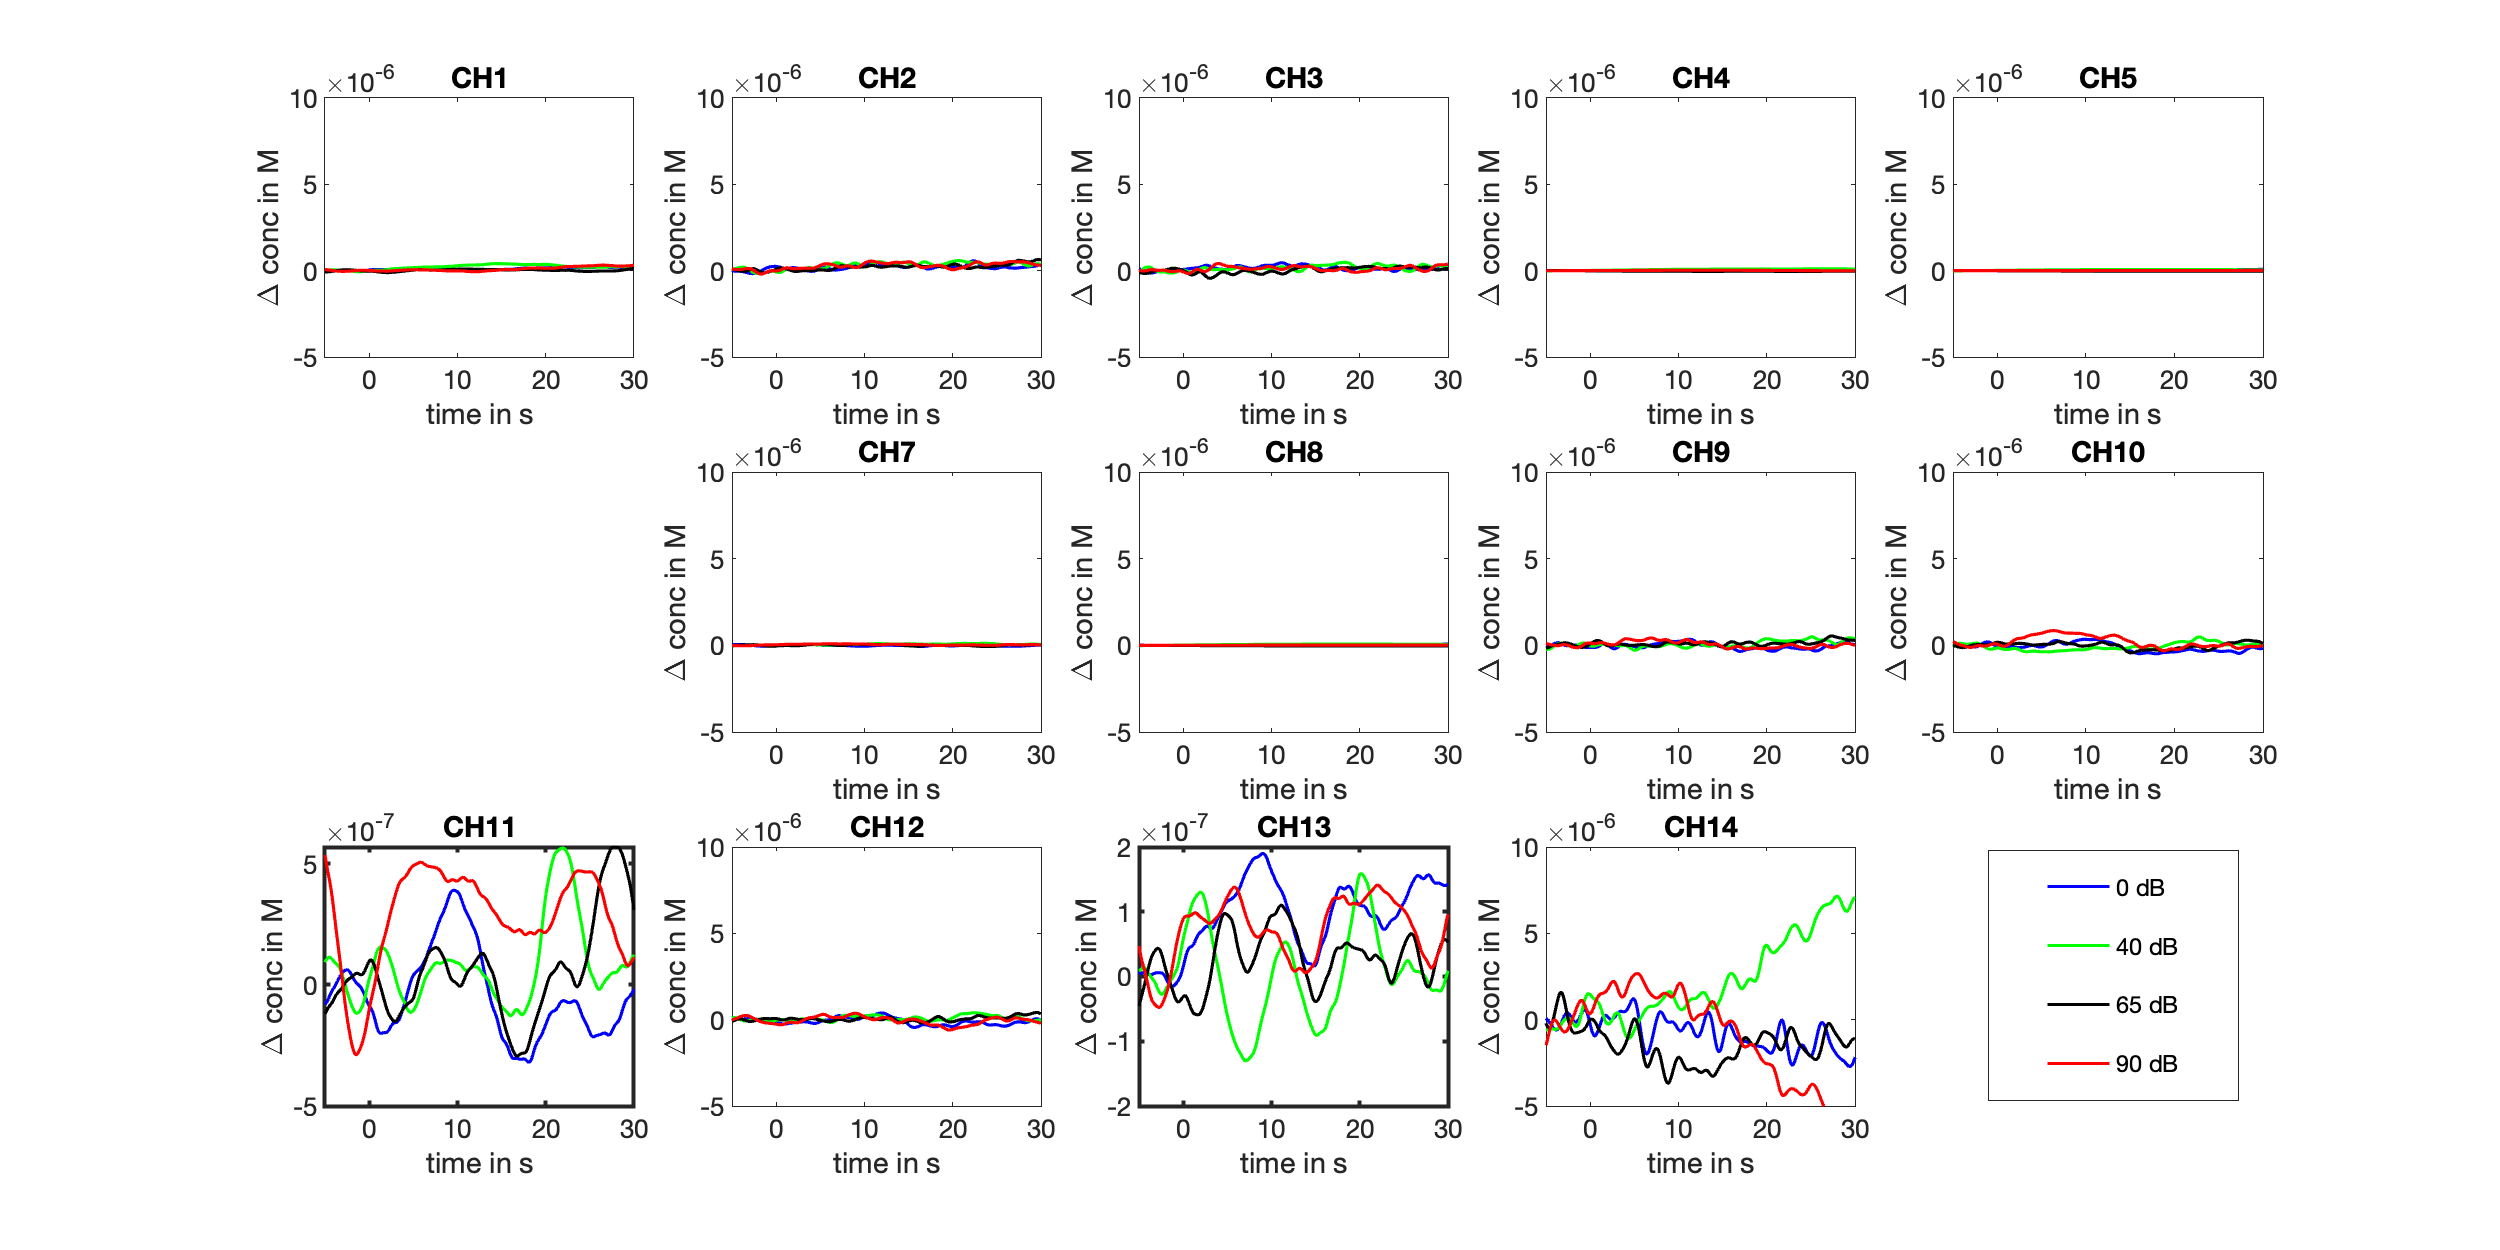
\includegraphics[scale=.35]{bilder/HbO_Mole/sub_lin_s_HbO.png}
  \caption{HbO Measurement from participant 4.}
  \medskip
  \footnotesize {Lines represent the block-averaged results over eight epochs. The averaged change of HbO concentration (in Mole) is plotted from 5 seconds before the start of the auditory stimuli to 30 seconds after the start of the stimuli. Four colours are used to differentiate the response from sound stimuli of different intensity levels.}
\end{figure}


\newpage


\begin{figure}[H]
  \centering
    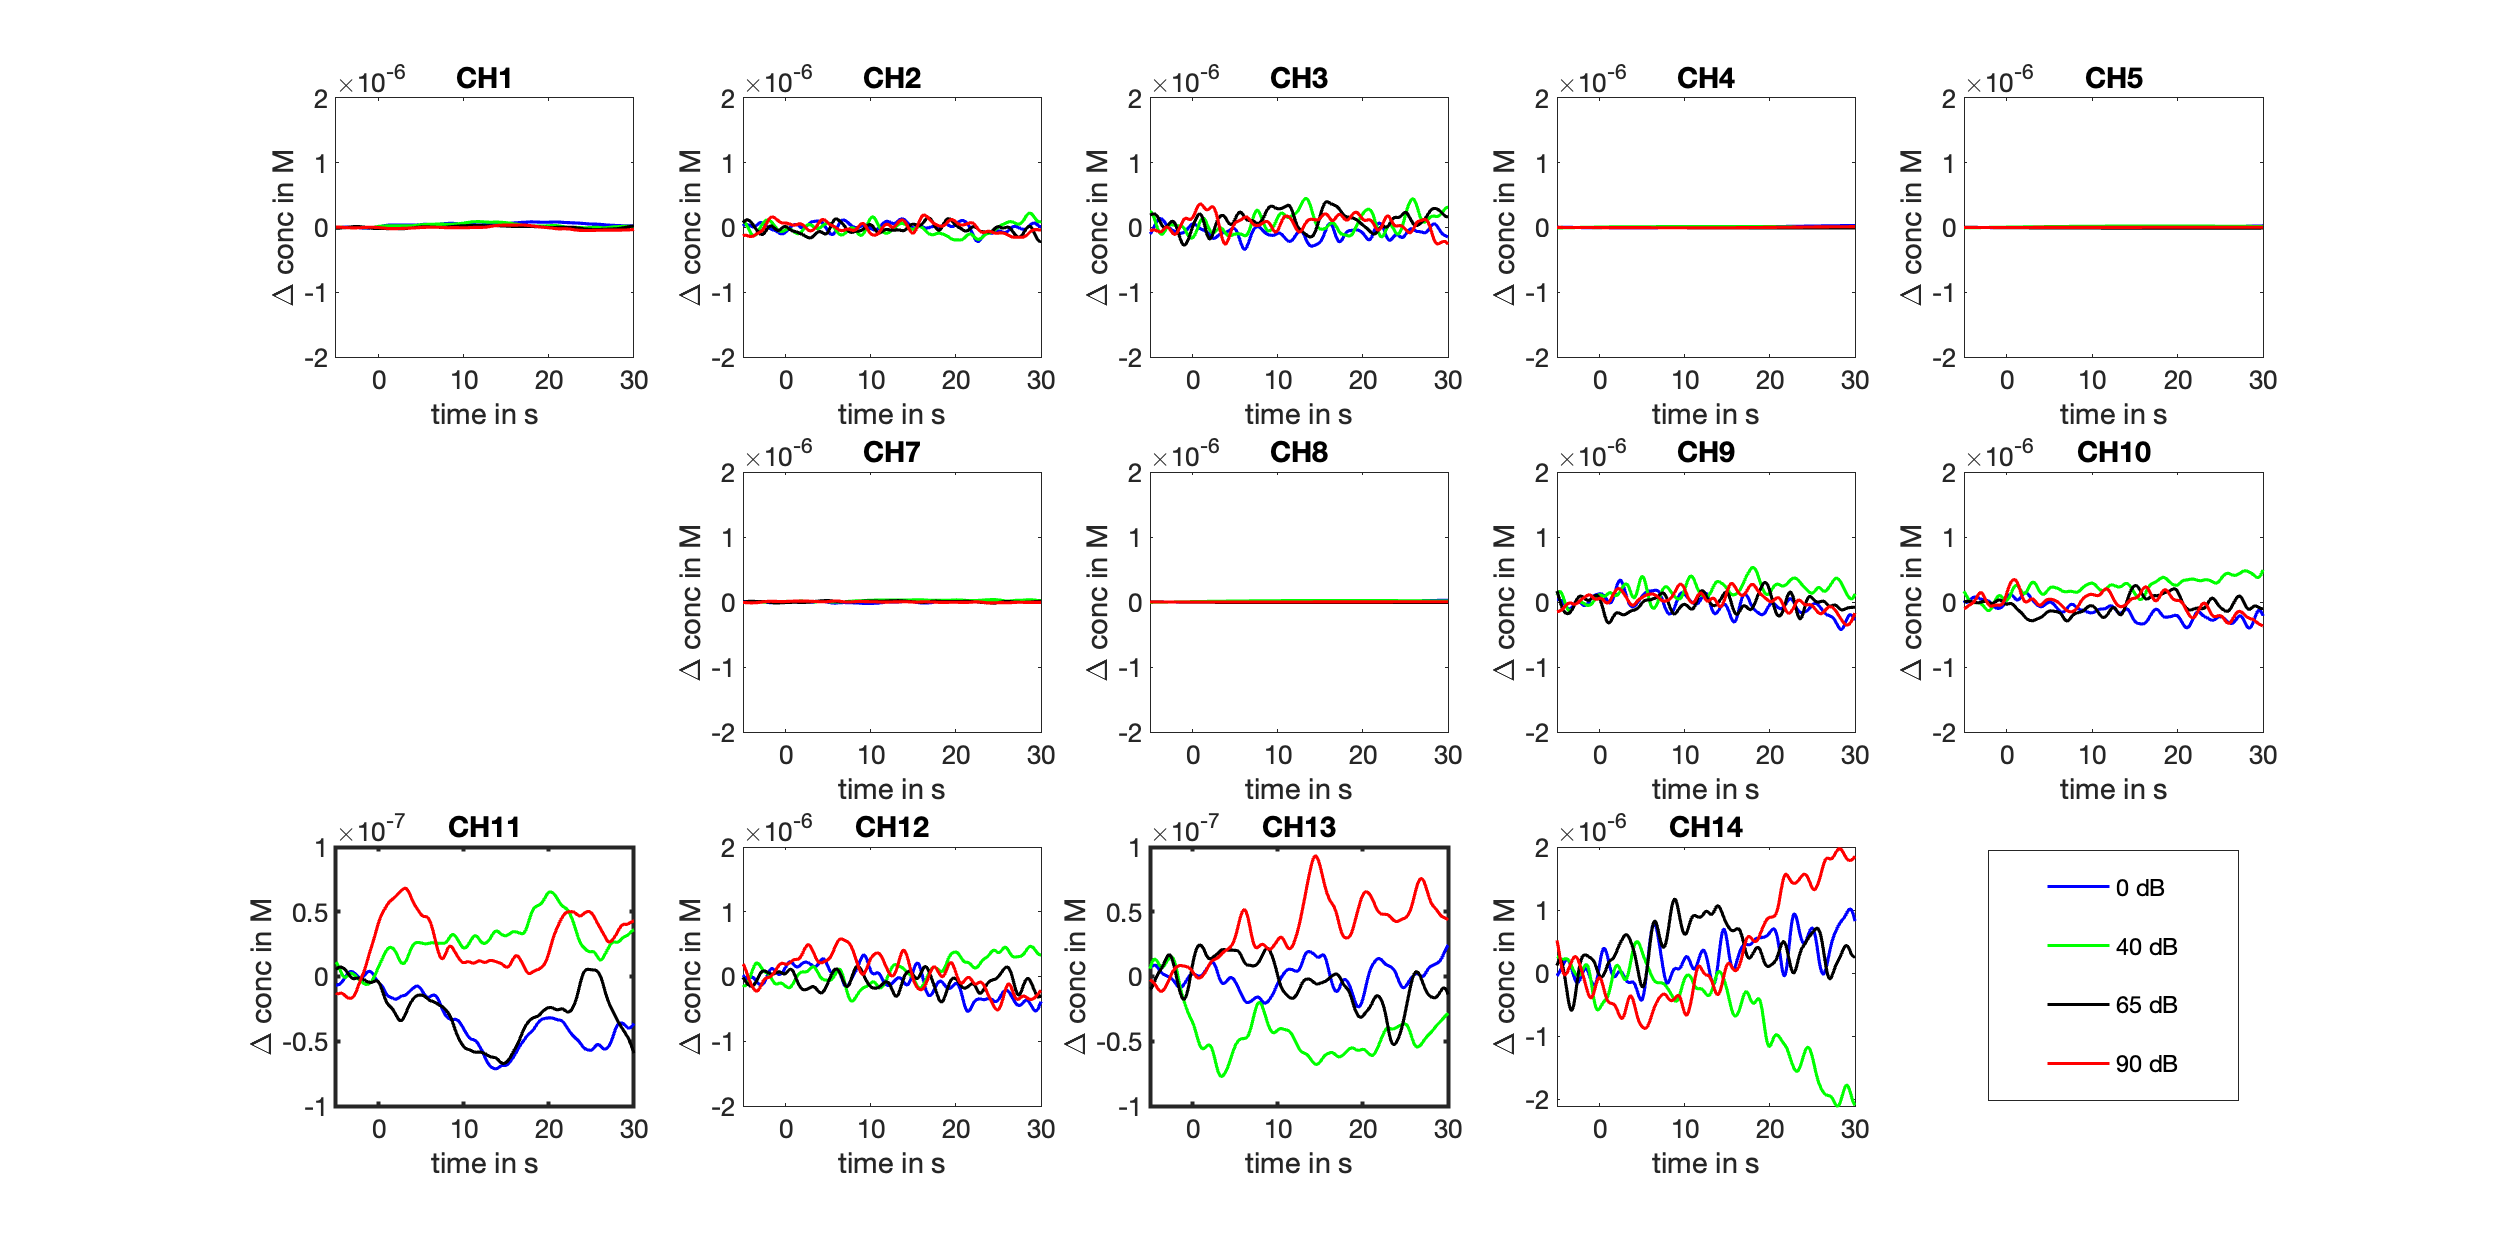
\includegraphics[scale=.35]{bilder/HbR_Mole/sub_lin_s_HbR.png}
  \caption{HbR Measurement from participant 4.}
  \medskip
  \footnotesize {Lines represent the block-averaged results over eight epochs. The averaged change of HbR concentration (in Mole) is plotted from 5 seconds before the start of the auditory stimuli to 30 seconds after the start of the stimuli. Four colours are used to differentiate the response from sound stimuli of different intensity levels.}
\end{figure}

\begin{figure}[H]
  \centering
    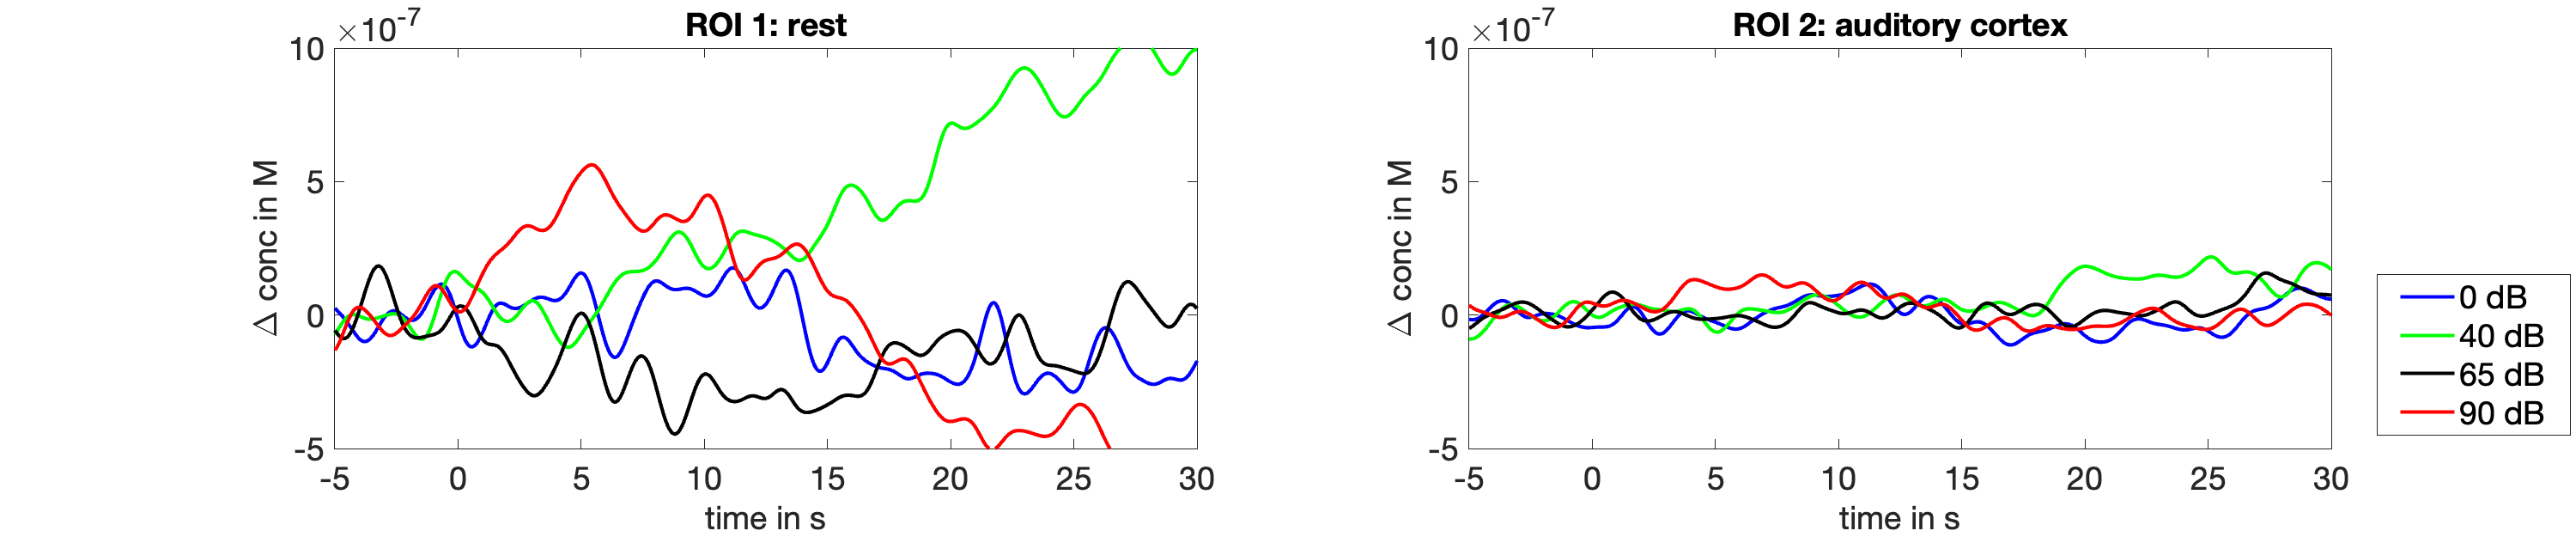
\includegraphics[scale=.29]{bilder/ROI/sub_lin_s_HbO.png}
  \caption{ROI Measurement from participant  4.}
\end{figure}

\newpage



\section {Participant 5}
\begin{figure}[H]
  \centering
    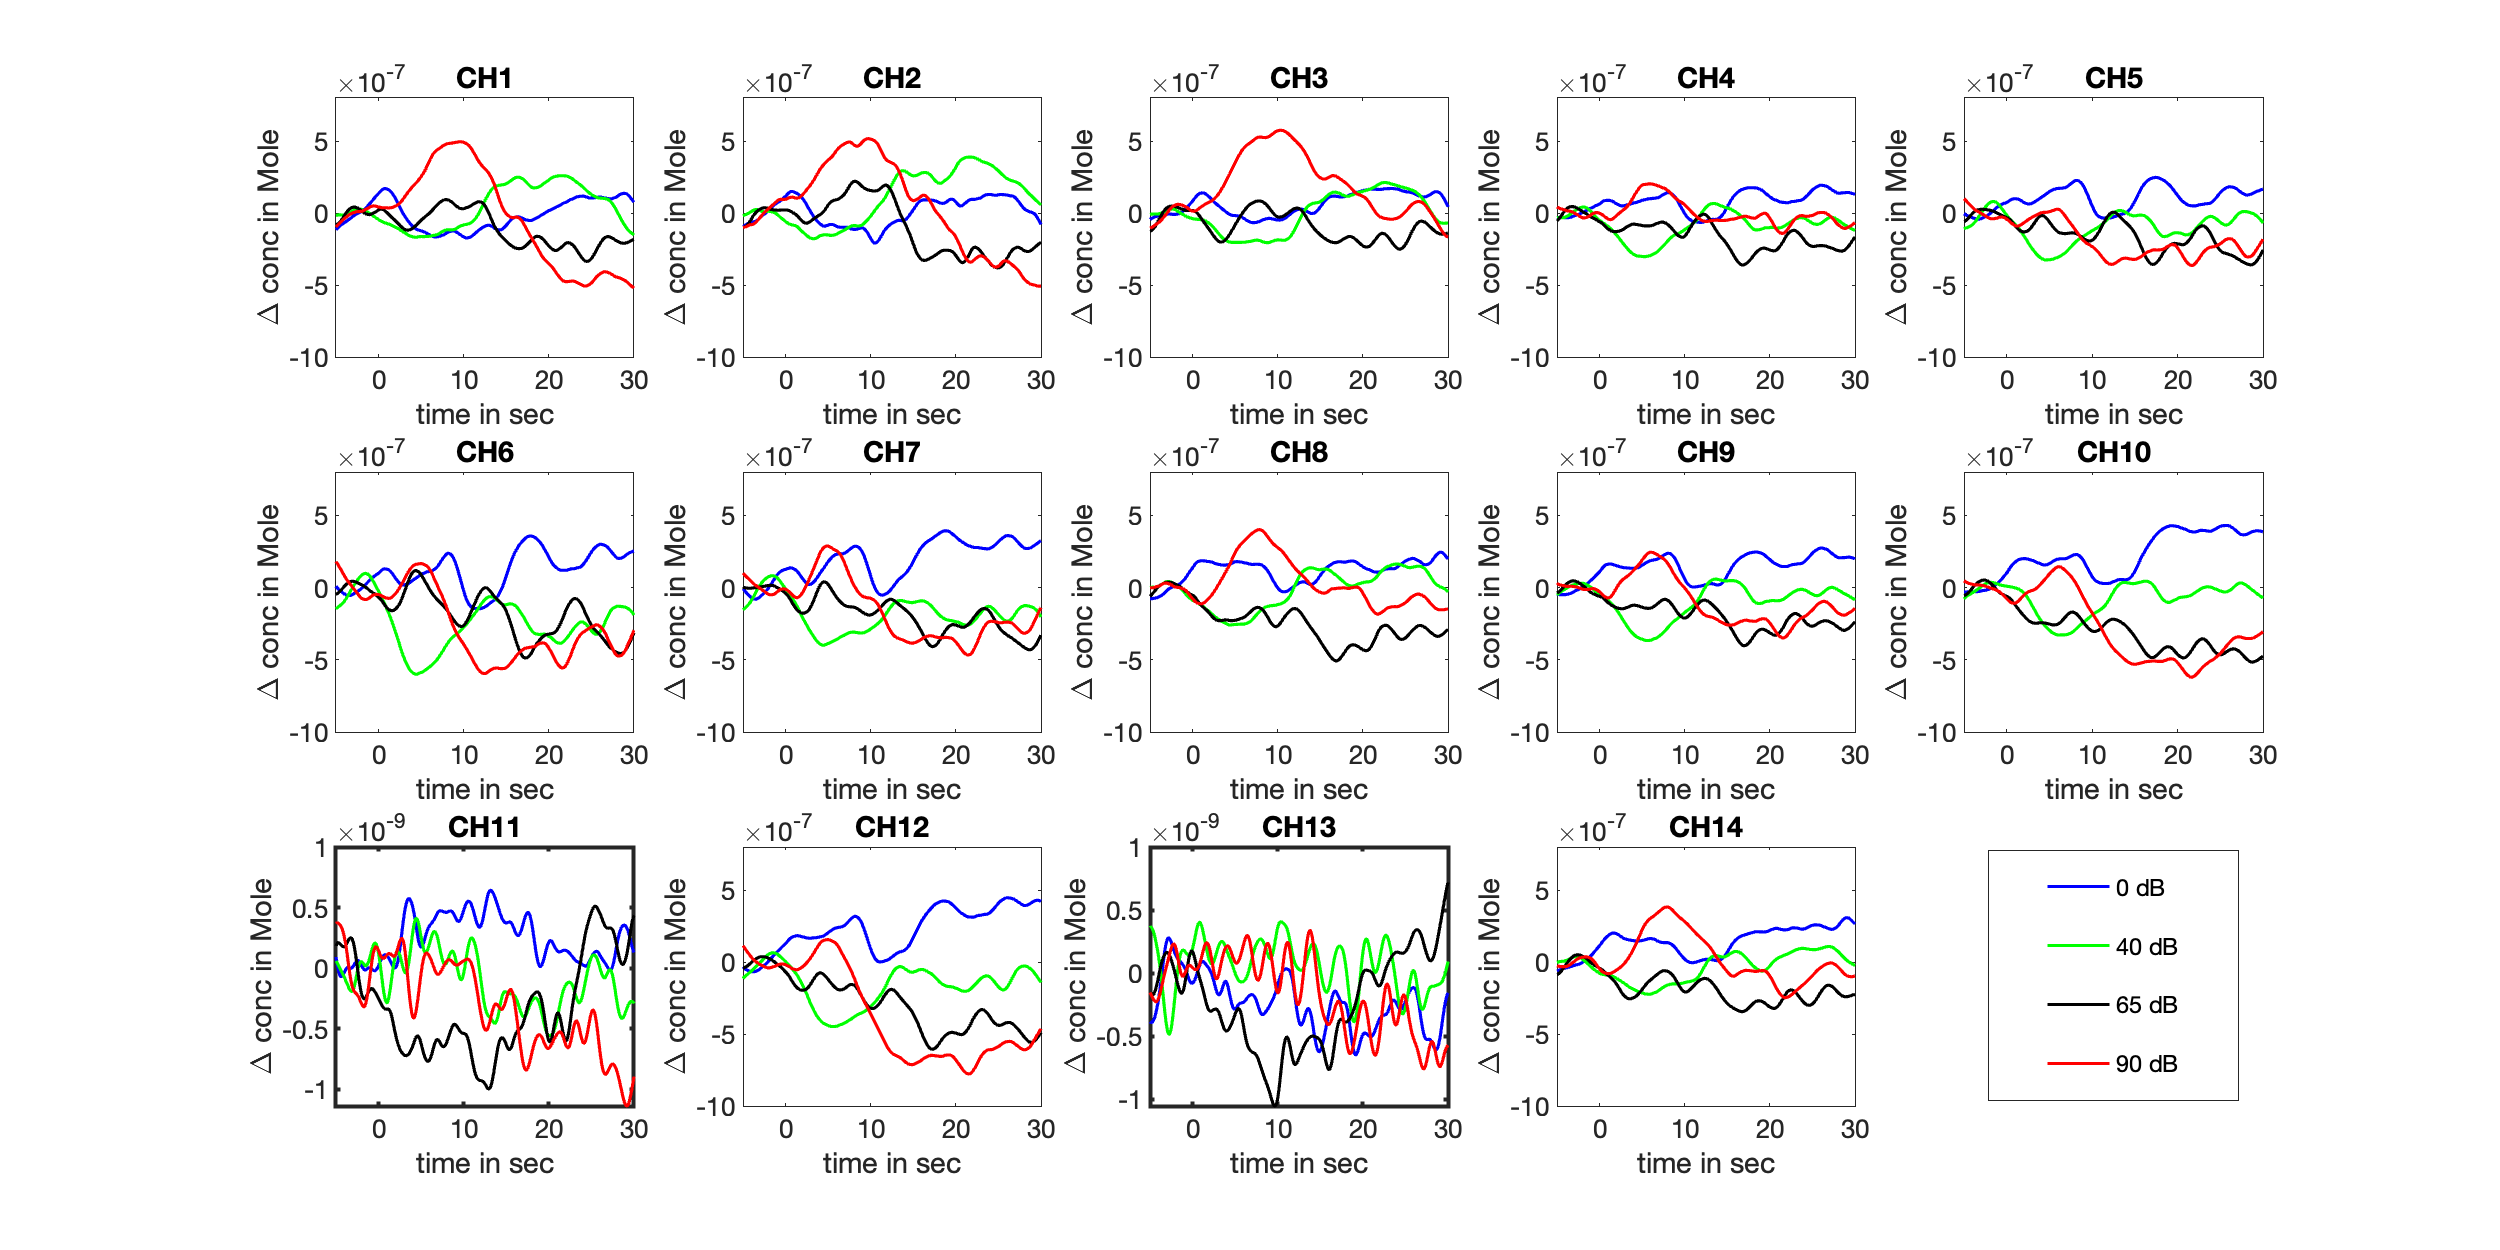
\includegraphics[scale=.4]{bilder/HbO_Mole/sub_lukas_s_HbO.png}
  \caption{HbO Measurement from participant 5.}
  \label{fig:somesignal}
  \medskip
  \footnotesize {Lines represent the block-averaged results over eight epochs. The averaged change of HbO concentration (in Mole) is plotted from 5 seconds before the start of the auditory stimuli to 30 seconds after the start of the stimuli. Four colours are used to differentiate the response from sound stimuli of different intensity levels.}
\end{figure}


\newpage


\begin{figure}[H]
  \centering
    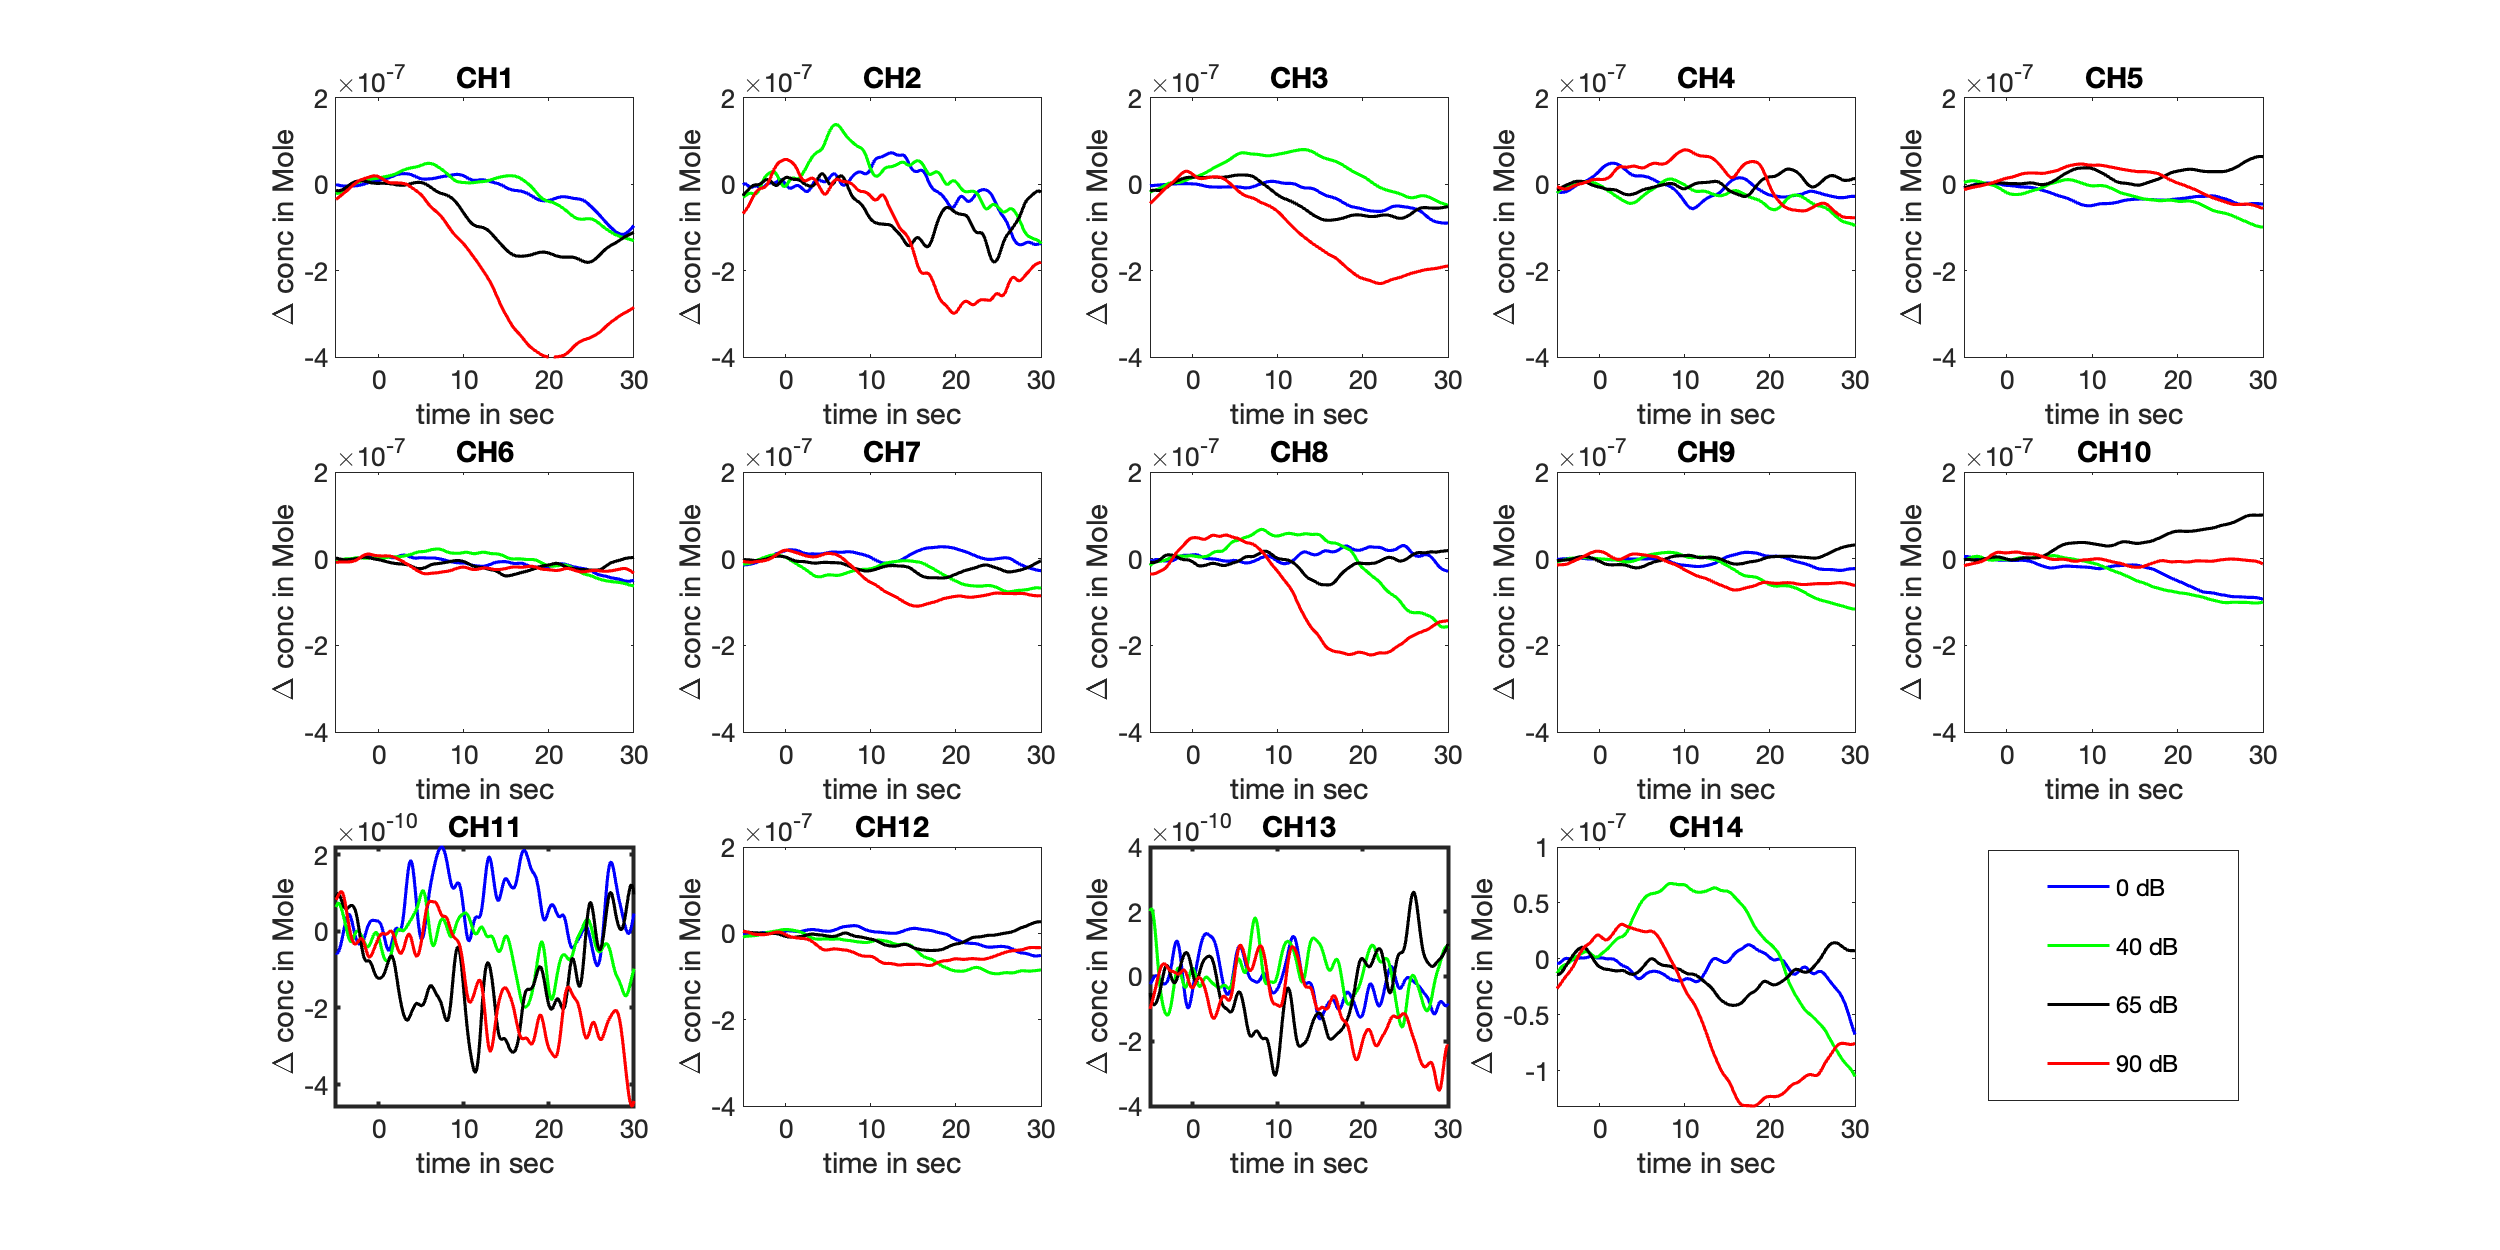
\includegraphics[scale=.4]{bilder/HbR_Mole/sub_lukas_s_HbR.png}
  \caption{HbR Measurement from participant 5.}
  \label{fig:somesignal}
  \medskip
  \footnotesize {Lines represent the block-averaged results over eight epochs. The averaged change of HbR concentration (in Mole) is plotted from 5 seconds before the start of the auditory stimuli to 30 seconds after the start of the stimuli. Four colours are used to differentiate the response from sound stimuli of different intensity levels.}
\end{figure}

\begin{figure}[H]
  \centering
    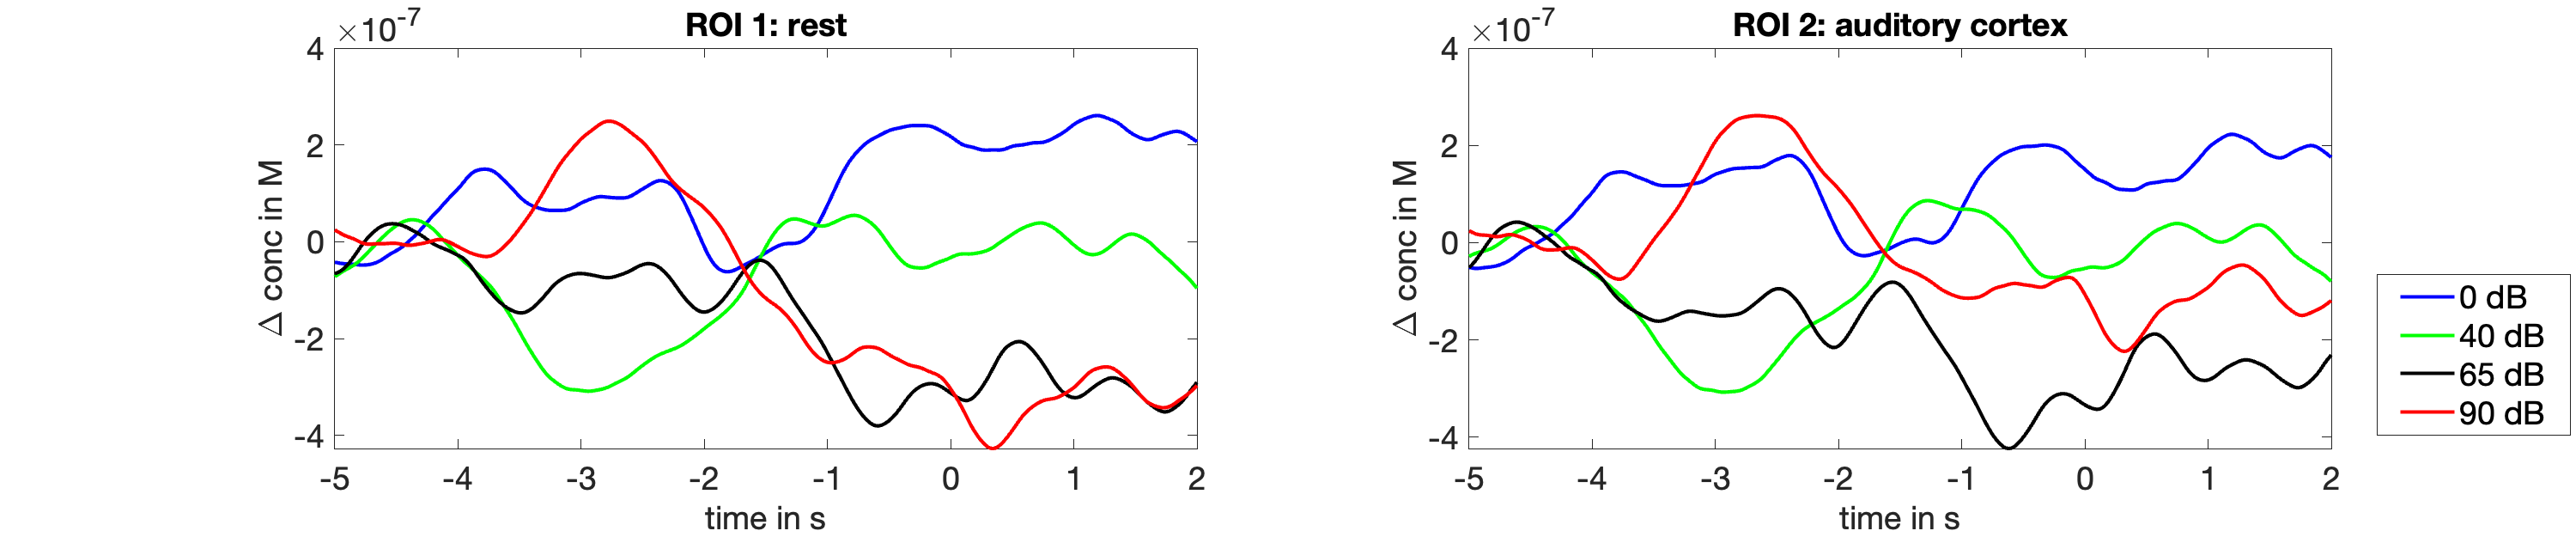
\includegraphics[scale=.29]{bilder/ROI/sub_lukas_s_HbO.png}
  \caption{ROI Measurement from participant 5.}
\end{figure}

For the \acrlong{HbO} (\acrshort{HbO} ) waveform, there were significantly larger on-sets for the 90 dB sound stimuli in Channel 1, 2, and 3, i.e. around the Broca's area.

Apart from this, the waveforms for \acrlong{HbR} (\acrshort{HbR}), were also quite different from the ones Weder et al \citeyearpar{Weder2018}. reported. For the loudest sound stimuli, channels overlying the caudal superior temporal gyrus and channels over Broca's area showed clear phasic response. 


\newpage





\section {Participant 7}
\begin{figure}[H]
  \centering
    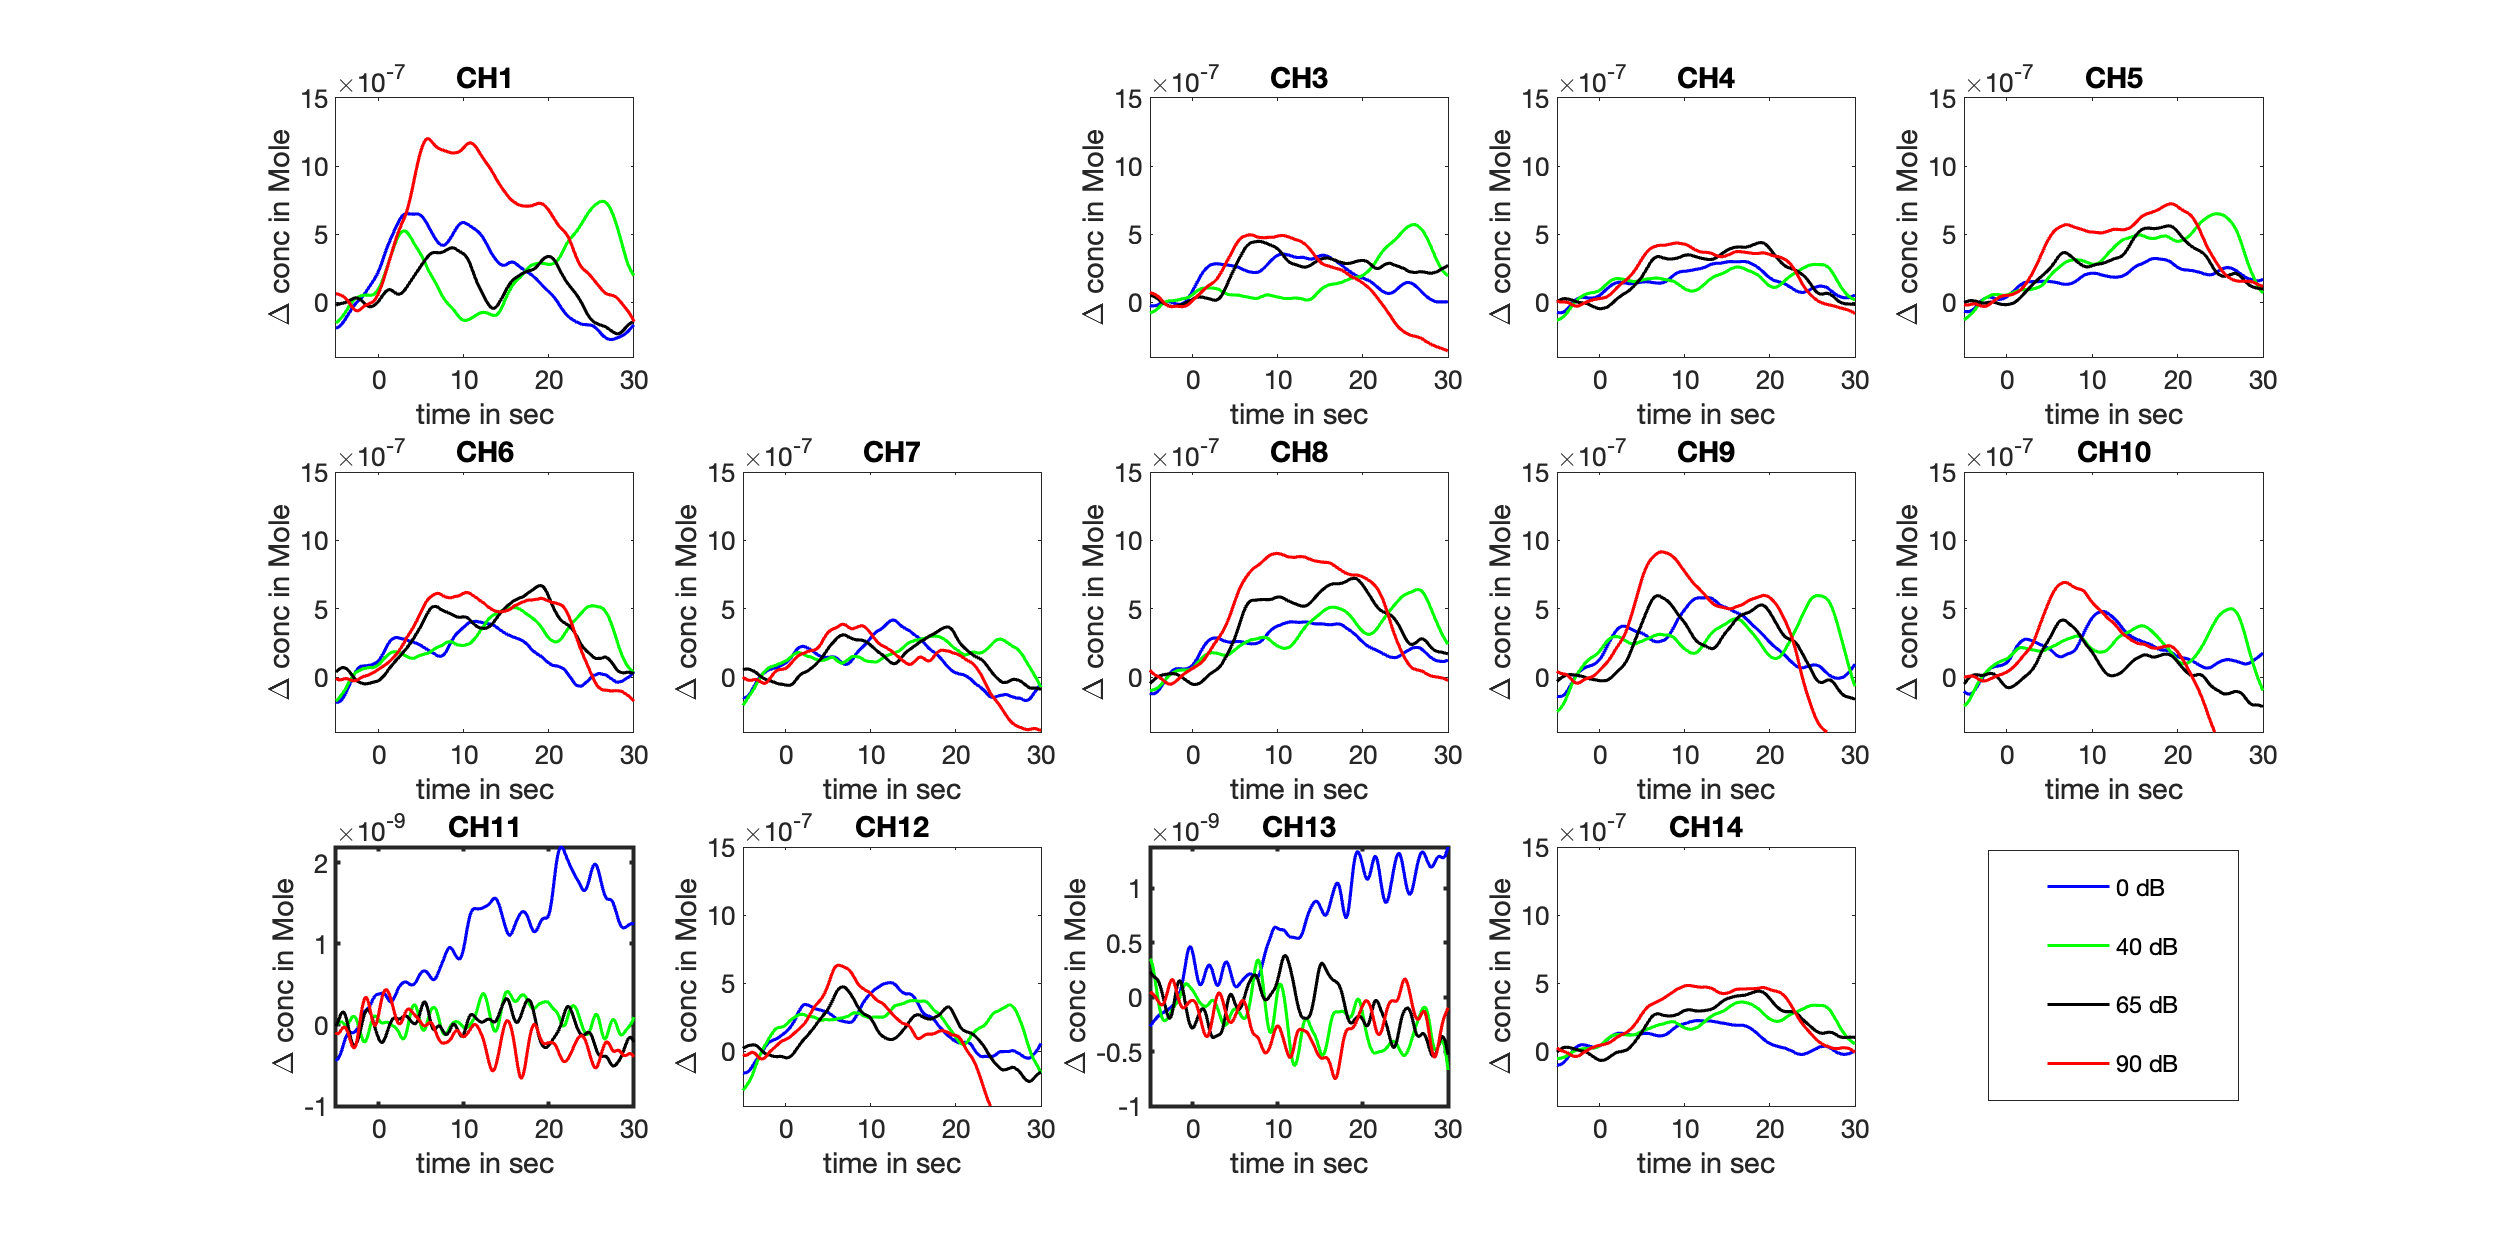
\includegraphics[scale=.4]{bilder/HbO_Mole/sub_liao_s_HbO.png}
  \caption{HbO Measurement from participant 7.}
  \label{fig:somesignal}
  \medskip
  \footnotesize {Lines represent the block-averaged results over eight epochs. The averaged change of HbO concentration (in Mole) is plotted from 5 seconds before the start of the auditory stimuli to 30 seconds after the start of the stimuli. Four colours are used to differentiate the response from sound stimuli of different intensity levels.}
\end{figure}


\newpage



\begin{figure}[H]
  \centering
    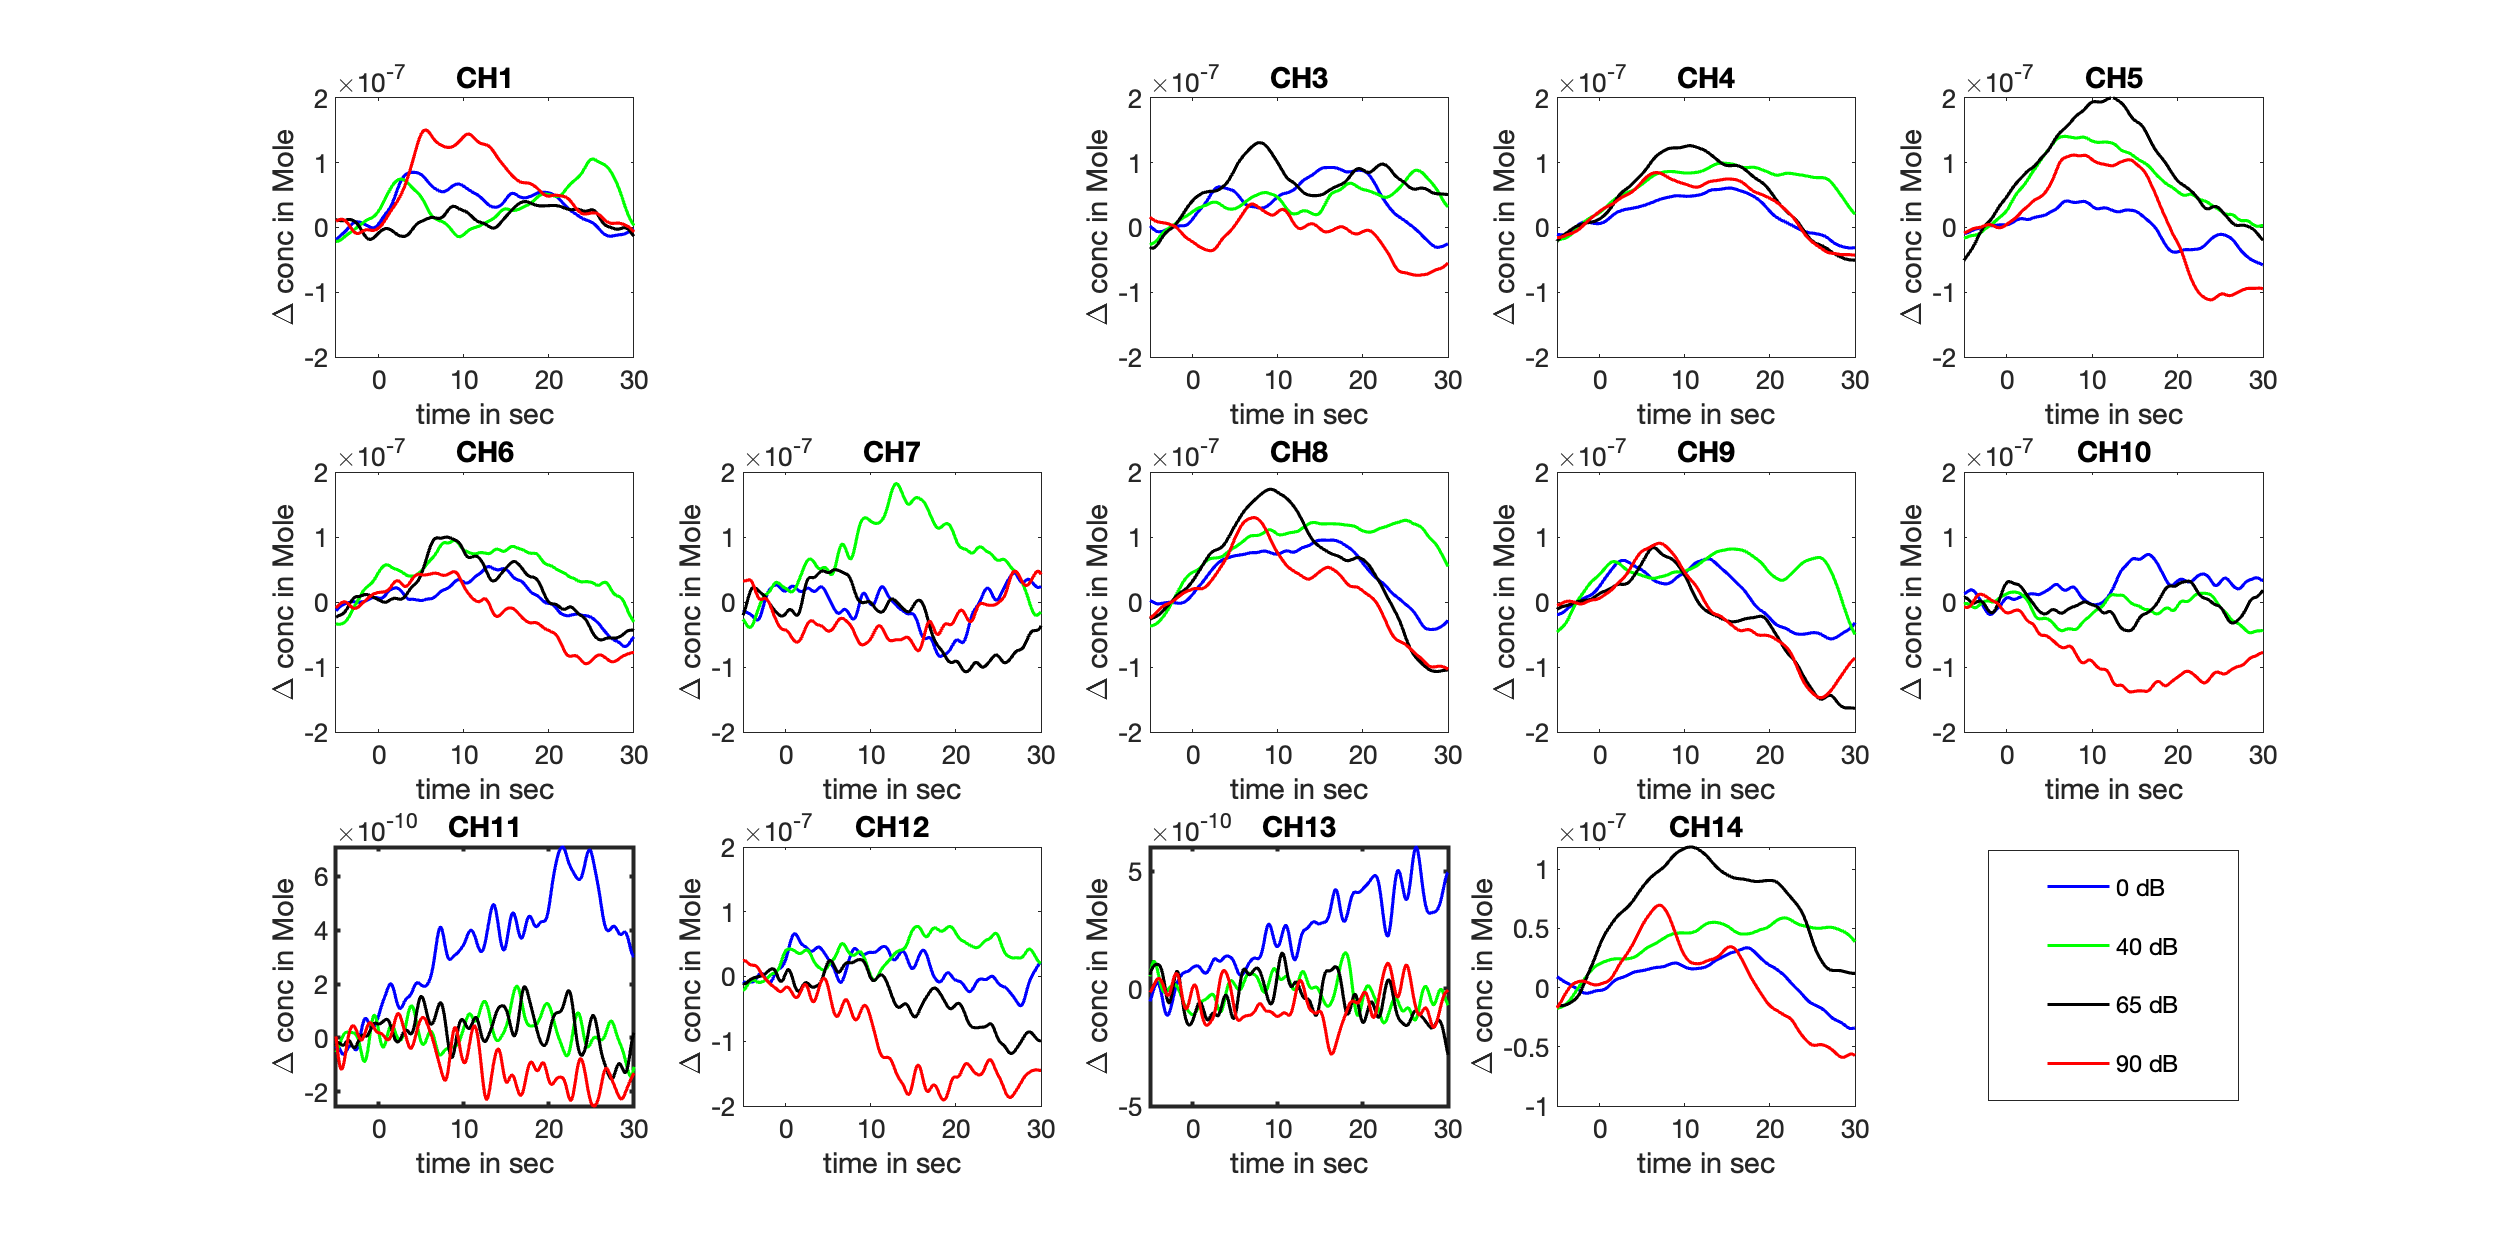
\includegraphics[scale=.4]{bilder/HbR_Mole/sub_liao_s_HbR.png}
  \caption{HbR Measurement from participant 7.}
  \label{fig:somesignal}
  \medskip
  \footnotesize {Lines represent the block-averaged results over eight epochs. The averaged change of HbR concentration (in Mole) is plotted from 5 seconds before the start of the auditory stimuli to 30 seconds after the start of the stimuli. Four colours are used to differentiate the response from sound stimuli of different intensity levels.}
\end{figure}

\begin{figure}[H]
  \centering
    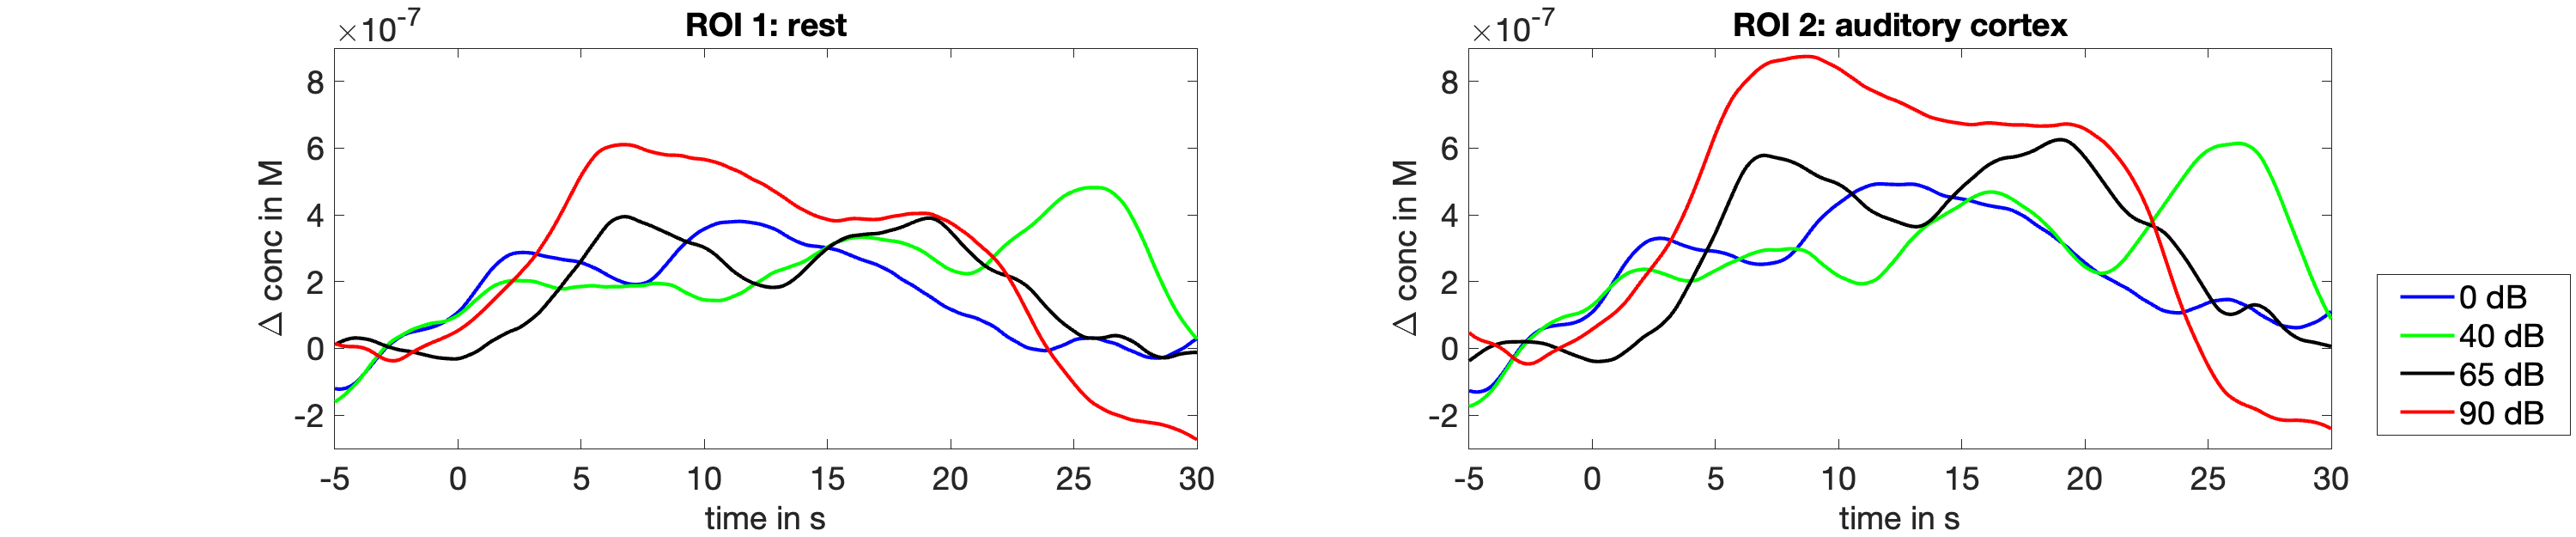
\includegraphics[scale=.29]{bilder/ROI/sub_liao_s_HbO.png}
  \caption{ROI Measurement from participant 7.}
\end{figure}

The results from this participant are rather indeterminant to differentiate between response to different sound pressure levels.

\newpage








%The following plots shows the averaged \textbf {HbO} response of all the valid channels in the defined region.

